\documentclass[a4paper,12pt]{article} 
\usepackage[T1]{fontenc}              
\usepackage[frenchb]{babel} % césures, titres français
\usepackage[utf8]{inputenc} % encodage
\usepackage[a4paper,left=3cm,right=3cm,top=2cm,bottom=2cm]{geometry} % marges
\usepackage{graphicx} % insertion d'images
\usepackage{rotating}
\usepackage{float} % permet d'utiliser H pour placer un flottant obligatoirement
\usepackage{pdfpages} % inclusion de PDF au sein du document
\usepackage{listings}
\pagestyle{plain} % pied de pages simples

\setlength{\parskip}{1ex plus 0.5ex minus 0.2ex} % espace entre les paragraphes
\setcounter{tocdepth}{2}
\setcounter{secnumdepth}{2}

\lstset{% general command to set parameter(s)
basicstyle=\ttfamily, % print whole listing small
keywordstyle=\color{black}\bfseries\underbar,
% underlined bold black keywords
identifierstyle=, % nothing happens
commentstyle=\color{white}, % white comments
showstringspaces=false,
numbers=left,
language=java,
breaklines=true,
frame=tblr} % no special string spaces

%%%% debut macro %%%%
\makeatletter
\renewcommand\section{\@startsection {section}{1}{\z@}%
                           {-3.5ex \@plus -1ex \@minus -.2ex}%
                           {2.3ex \@plus.2ex}%
                           {\normalfont\Large\bfseries}}
\makeatother
%%%% fin macro %%%%



% Def
\newcommand{\code}[1]{{\lstinline{#1}}}

\begin{document}
\newpage
\title{J2EE\\TP2}
\date{}
\author{BRIZAI Olivier\\THORAVAL Maxime}
\maketitle

\newpage
\section{Architecture de l'application}
L'architecture de notre application ressemble traits pour traits à celle décrite dans le sujet du TP.\\
C'est ainsi que nous retrouvons :
\begin{itemize}
	\item Le package ensicaen.tb.mvc.eleves.dao. Contient DAOException, DAOImpl et IDAO.
	\item Le package ensicaen.tb.mvc.eleves.entities. Contient la classe Eleve.
	\item Le package ensicaen.tb.mvc.eleves.service. Contient IService et IServiceImpl.
	\item Le package ensicaen.tb.mvc.eleves.test. Contient TestDAO et TestService.
	\item Le package ensicaen.tb.mvc.eleves.web. Contient Application.
	\item Le dossier WEB-INF/vues. Contient les vues edit, erreurs, exception et list.
\end{itemize}
~\\

Pour rendre notre application plus fonctionnelle est plus ergonomique, nous nous sommes permis d'utiliser le framework \textit{Blueprint}.
Celui-ci permet de générer rapidement et efficacement une interface web. Celui-ci est ainsi situé dans le dossier \textit{blueprint}.\\
Dans la même perspective, nous avons rajouter des icônes permettant de différencier facilement l'ajout, la modification et la suppression. 
Ceux-ci sont visible dans le dossier \textit{icons}.\\
Enfin, nous avons rajouter une page par défaut pour les erreurs de type 404. Celle-ci contient simplement une image (dossier \textit{icons}) et
un lien vers la liste des élèves.


\begin{figure}[H]
	\center
	\fbox{
	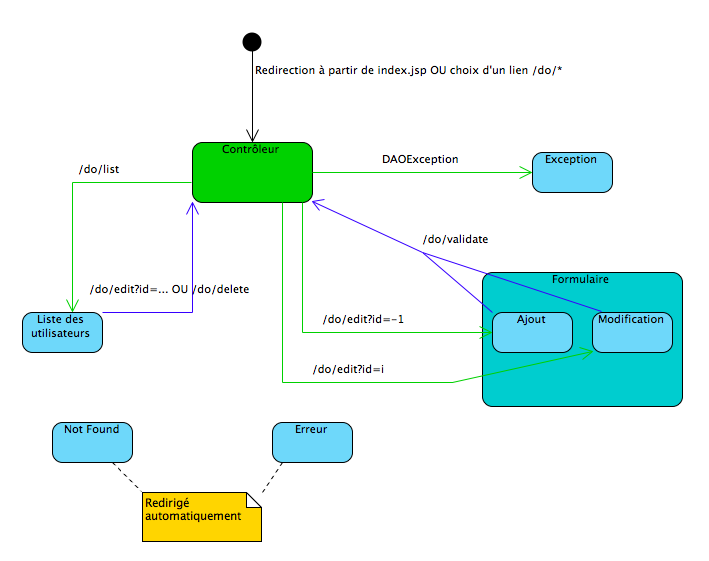
\includegraphics[width=15cm]{img/archi.png}
	}
	\caption{Architecture de l'application}
\end{figure}

\section{Les différentes pages}
\subsubsection{Liste des élèves}	
	\begin{figure}[H]
		\center
		\fbox{
		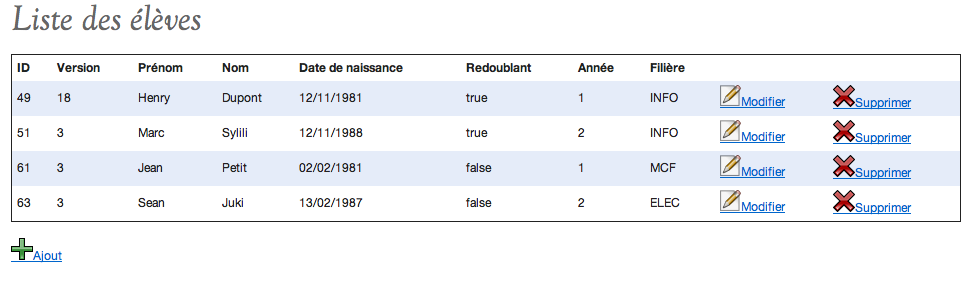
\includegraphics[width=15cm]{img/list.png}
		}
		\caption{Liste des élèves}
	\end{figure}

\subsubsection{Ajout}
	\begin{figure}[H]
		\center
		\fbox{
		
\includegraphics[width=15cm]{img/add.png}
		}
		\caption{Ajout d'un élèves}
	\end{figure}
	
\subsubsection{Modification}
	\begin{figure}[H]
		\center
		\fbox{
		
\includegraphics[width=15cm]{img/edit.png}
		}
		\caption{Modification d'un élèves}
	\end{figure}

\subsubsection{Mauvais champs lors de l'ajout/modification}
	\begin{figure}[H]
		\center
		\fbox{
		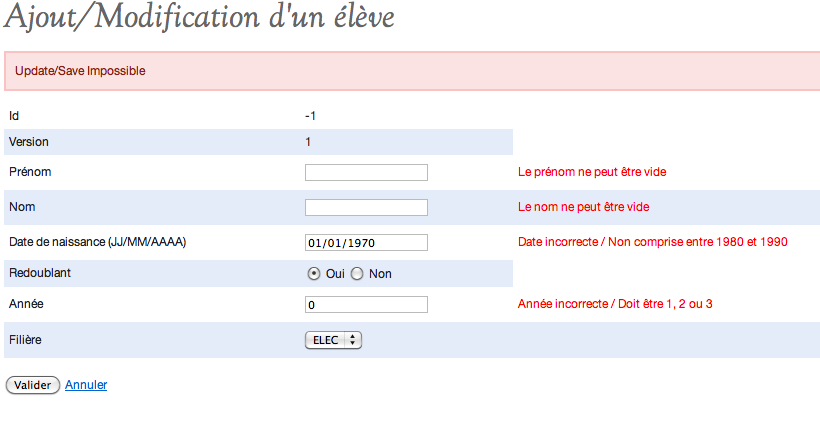
\includegraphics[width=15cm]{img/addwitherror.png}
		}
		\caption{Problèmes lors du renseignement des informations}
\end{figure}
	

\subsubsection{Exceptions}
	\begin{figure}[H]
		\center
		\fbox{
		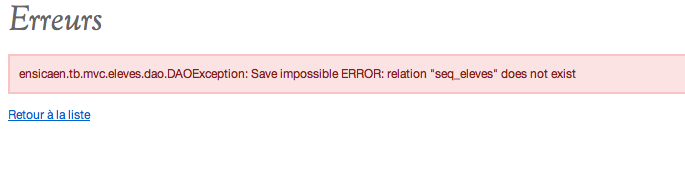
\includegraphics[width=15cm]{img/exception.png}
		}
		\caption{Page d'exception}
	\end{figure}
	
	
\subsubsection{Erreurs}
Nous avons considéré que si cette page apparaissait, cela signifiait que l'erreur était importante.
Cela explique le fait qu'il n'y ait aucun lien vers une autre page.
	\begin{figure}[H]
		\center
		\fbox{
		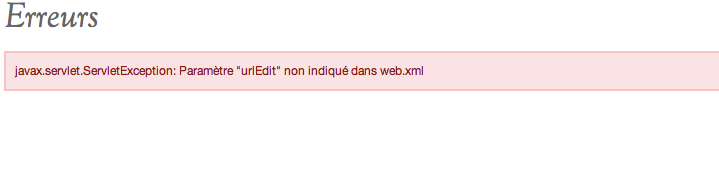
\includegraphics[width=15cm]{img/error.png}
		}
		\caption{Page d'erreur}
	\end{figure}

	
\subsubsection{Non trouvé}
	\begin{figure}[H]
		\center
		\fbox{
		
\includegraphics[width=10cm]{img/notfound.png}
		}
		\caption{Page de \og Non trouvé \fg}
	\end{figure}

\section{Tableau des erreurs}

\begin{tabular}{|l|c|}
  \hline
  Numéro & Type d'erreur \\
  \hline
	10 & Impossible de charger le driver \\
	11 & Problème lors de la connexion à la base de données \\
	12 & Problème lors de la préparation des statements \\
 	13 & Problème lors de la fermeture de la connexion à la BDD \\
	20 & Problème lors de la recherche de la liste totale des élèves dans la BDD \\
	30 & Problème lors de le recherche de l'ID d'un élève dans la BDD\\
	31 & Pas de résultat dans la recherche de l'ID d'un élève dans la BDD \\
	40 & Update/Save impossible, problème dans les informations fournies pour l'élève \\
	41 & Problème lors de la sauvegarde dans la BDD \\
	42 & Problème lors de la mise à des informations d'un élève dans la BDD\\
	43 & Update impossible, version de l'élève invalide (problème de synchronisation)\\
	50 & Problème lors de la suppression d'un élève \\
  \hline
\end{tabular}
~\\

Nous avons modifié la classe \textit{DAOException} par rapport à celle fournie dans le sujet.\\
En effet, nous avons remarqué que pour gérer les problèmes d'ajout/mise à jour (code 40) d'un élève,
un simple code n'était pas suffisant et nécessitait d'autres tests dans le contrôleur. Un tableau de codes
d'erreur a ainsi été crée. Chaque code est associé à une donnée qui est mal renseignée. Le contrôleur ne se charge
alors que de \og mettre un texte \fg sur ceux qu'il reçoit.\\

\begin{tabular}{|l|c|}
  \hline
Numéro & Type d'erreur \\
  \hline
	1 & Objet Eleve vide \\
	2 & Aucun nom de renseigné \\
	3 & Aucun prénom de renseigné \\
	4 & Filière non renseignée ou non existante \\
	5 & Date incohérente ou non comprise en 1980 et 1990\\
	6 & Année non renseignée ou non comprise entre 1 et 3 \\
  \hline
\end{tabular}


\end{document}


